\documentclass{myBook}

\title{Maths for Economists: A Comprehensive Handbook}
\author{Zhenran Guo}
\date{\today}


\begin{document}

% Front matter section.
\frontmatter

% Include the title page, which is located in the FrontMatter subfolder.
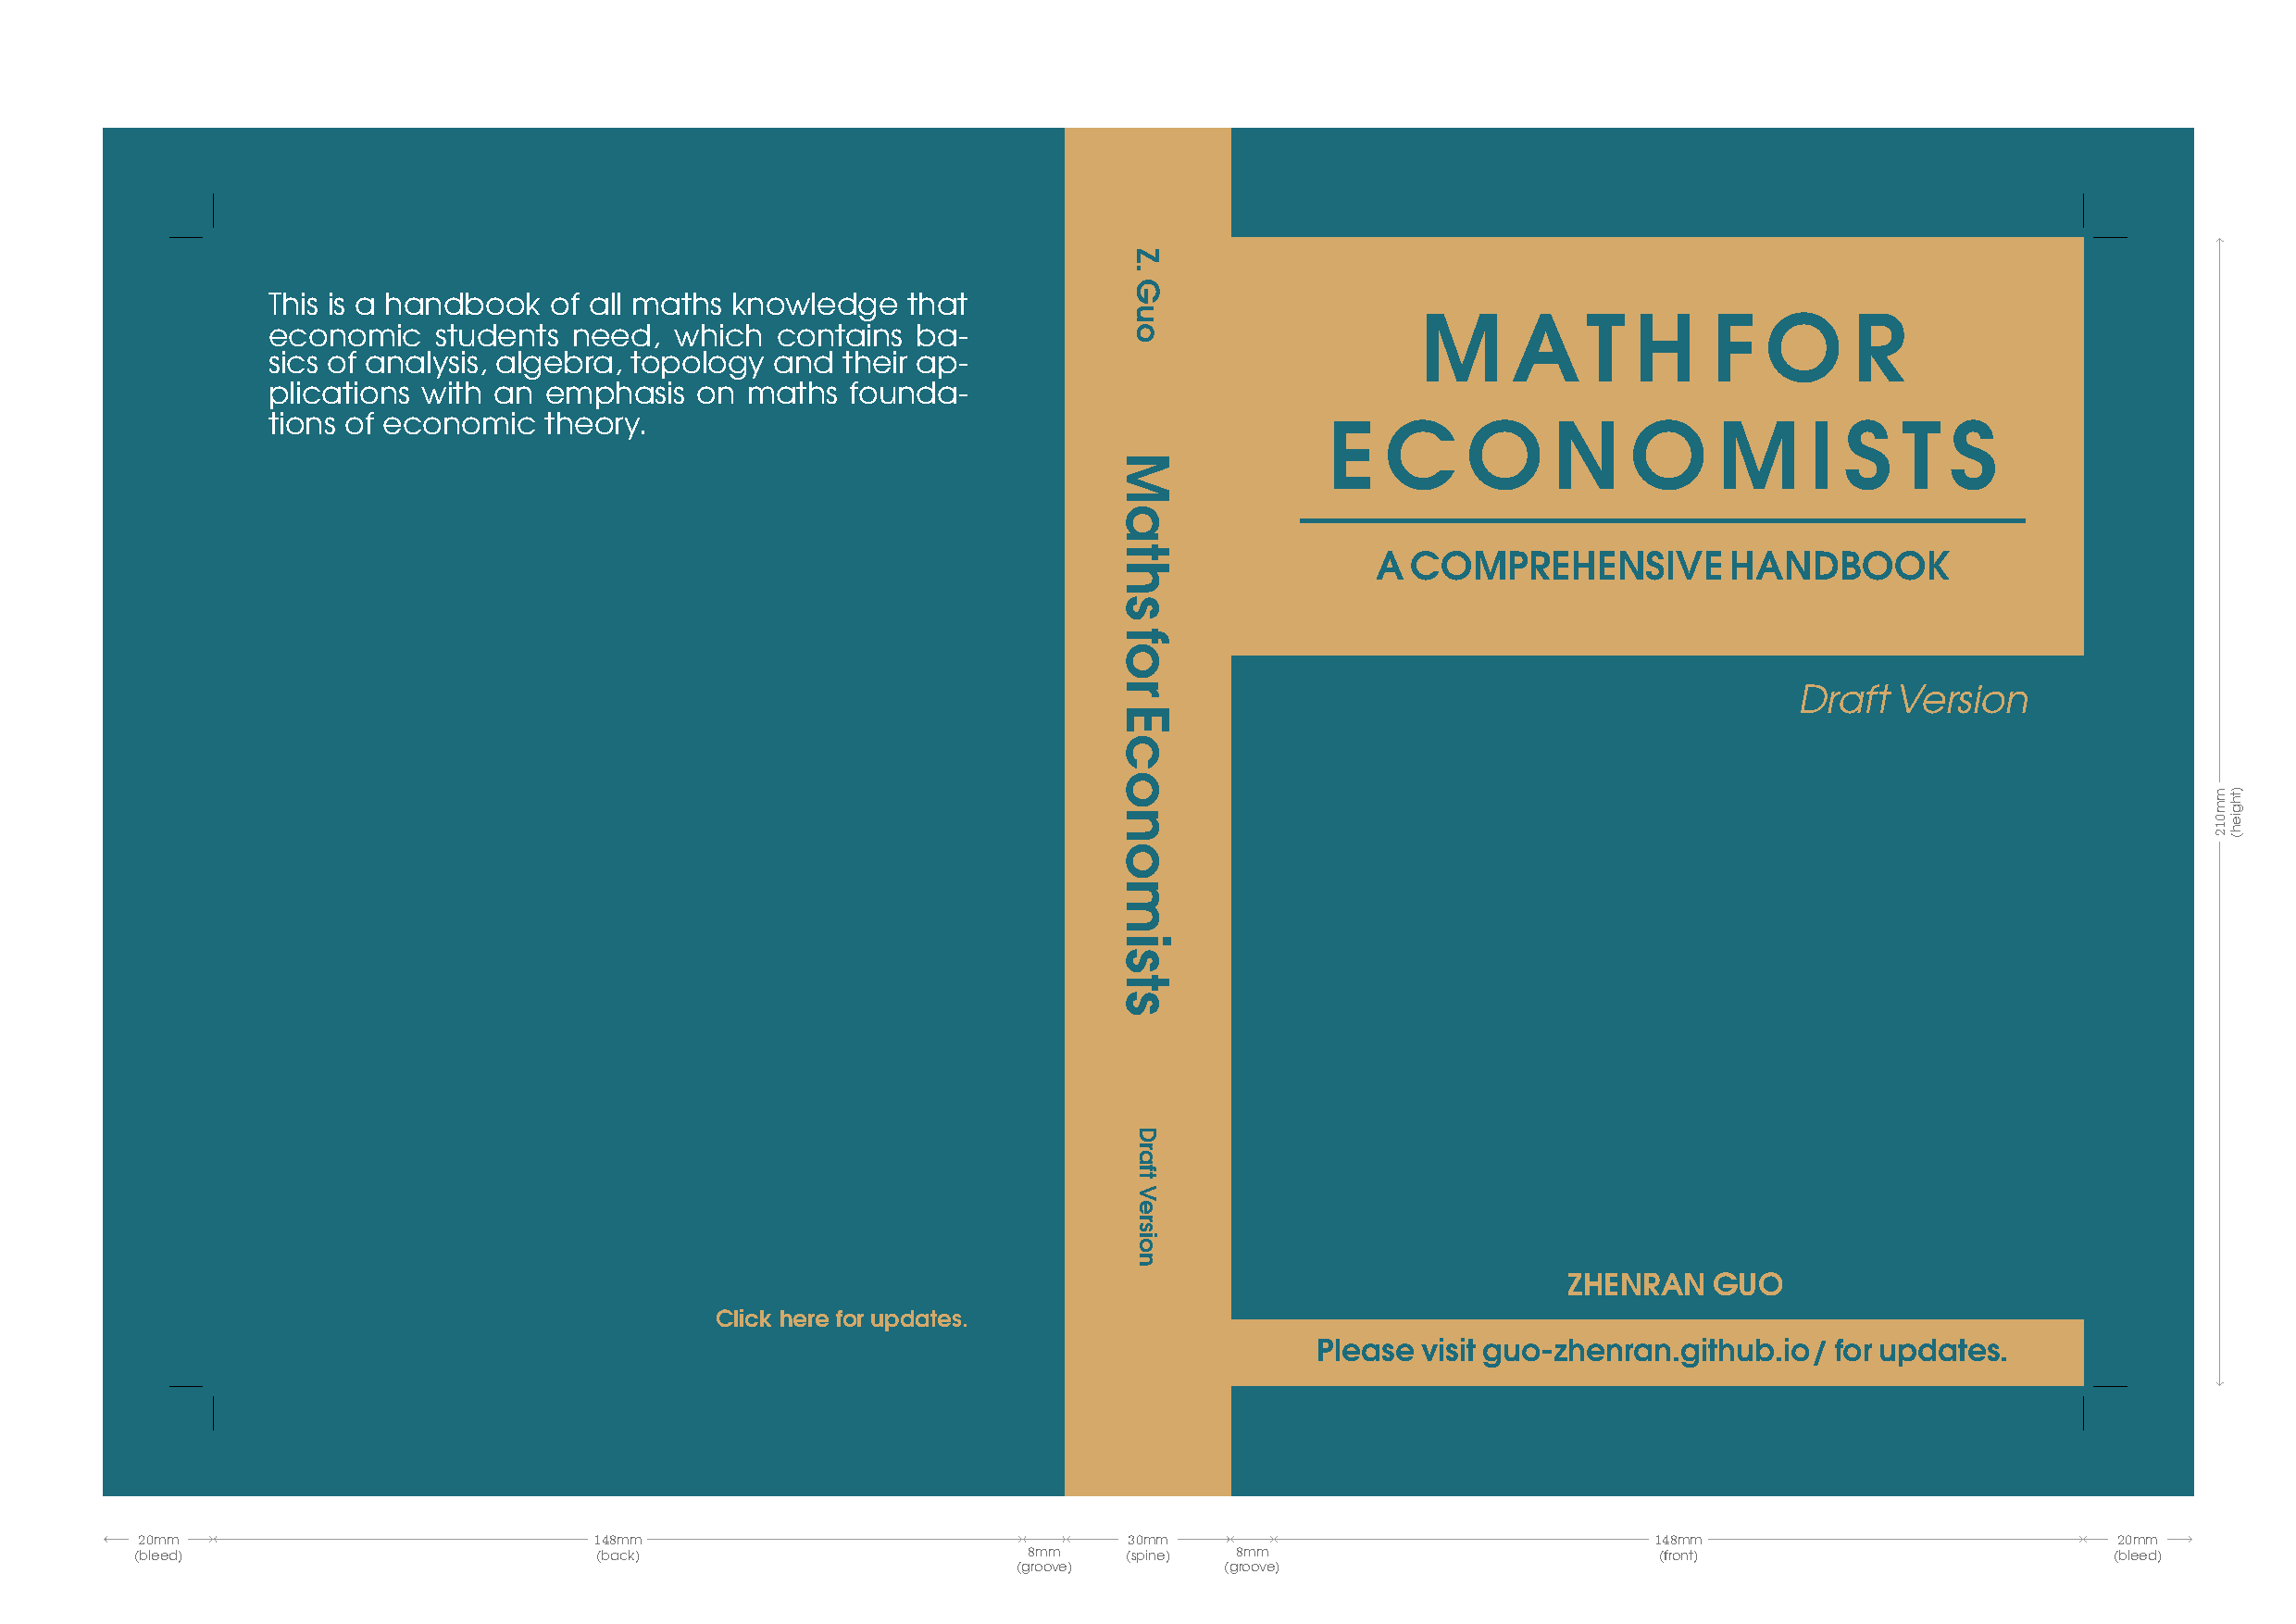
\includepdf[pages={1}]{./FrontMatter/BookCover/Cover.Maths-for-Economists.pdf}

% Create the book's title page.
\maketitle\pagebreak

% Include the preface page from the FrontMatter subfolder.
\input{./FrontMatter/preface}

% Include the acknowledgement page from the FrontMatter subfolder.
\chapter*{Acknowledgement}
This book is written using \LaTeX. The template is based on Agni Datta's \href{https://www.overleaf.com/latex/templates/preprint-book-manuscript-template/ghrbwppzhzjx}{"Preprint Book Manuscript Template"}, which I have modified to fit my requirements. 
The famous \href{https://github.com/ElegantLaTeX/ElegantLaTeX}{ElegantLaTeX} template has also inspired me greatly. The source code is available in \href{https://github.com/guo-zhenran/Maths-for-Economists}{my GitHub repository} for reference.

My best greetings go to \href{https://minamomo127430.github.io/}{Zhihao Hu} (SJTU), without whose constructive advice the completion of this book would have been impossible. I would also like to thank Copilot and DeepSeek for helping me write and edit this book. 

% Table of contents page.
\tableofcontents

% Main matter section.
\mainmatter

% Part 1: Foundations.
\part{Foundations}
\input{./MainMatter/Foundations/Logic}

\input{./MainMatter/Foundations/Intro_to_Set}
\input{./MainMatter/Foundations/Set_Theory}

\input{./MainMatter/Foundations/Relation_and_Operation}

\input{./MainMatter/Foundations/Countability}

\chapter{Group, Ring and Field}
\input{./MainMatter/Foundations/Group.tex}
\input{./MainMatter/Foundations/Ring&Field.tex}
\input{./MainMatter/Foundations/Polynomials.tex}

\part{Vector Space and Linear Algebra}
\input{./MainMatter/Vector Space and Linear Algebra/Vec_spc}
\input{./MainMatter/Vector Space and Linear Algebra/Linear_mapping.tex}
\input{./MainMatter/Vector Space and Linear Algebra/Normed_vecspc}
\input{./MainMatter/Vector Space and Linear Algebra/Multilinear_Form}
\input{./MainMatter/Vector Space and Linear Algebra/Eigenvalue_and_Eigenvector}

\part{Metric Space and Topology Space}
\input{./MainMatter/Metric Space and Topology Space/Metric_spc.tex}
\input{./MainMatter/Metric Space and Topology Space/Top_spc.tex}

\part{Measure, Integration and Differentiation}


\part{Probabilistic Theory and Basics in Statistical Inference}


\part{Tools in Economics}
\chapter{Optimization}
\section{Analysis on Covex Sets}
\subsection{Convex Set}
Recall the definition of linear combination:
$$\forall x,y \in V, a,b \in \mathbb{F}: ax+by.$$
If we further restrict $a+b=1$, we say it's a convex combination. 
\begin{definition}[Convex Set]
    Let $W$ be a subset of $V$, we say it's a convex subset if $W$ is closed under convex combination. We denote convex hull, the smallest convex set containing $W$, as $co(W)$, i.e.,
    $$co(W):=\bigcap\{C: C \text{ is convex } \land W\subset C\}.$$ 
\end{definition}
\subsection{Convex Functions}
\begin{definition}[Convex and Concave Functions]
    Suppose $C$ is a convex set, we say $f: C\to V$ to $V$ is (strictly) convex if and only if 
$\forall x,y\in C$ and $a\in [0,1]$, $$f(ax+(1-a)y) (<)\leq af(x)+(1-a)f(y).$$
\,If $-f$ is (strictly) convex, we say $f$ is (strictly) concave.
\end{definition}

We now turn studying whether a function is convex to studying whether a set is convex.
\begin{definition}
    We define the following:
    \begin{description}
        \item[Epigraph] $Epi(a):=\{(x,a) \in X\times \R: a\geq f(x)\}$
        \item[Subgraph] $Sub(a):=\{(x,a) \in X\times \R: a\leq f(x)\}$
    \end{description}
\end{definition}

\begin{proposition}
    Suppose $f:C\to \R$, then 
    \begin{itemize}
        \item $f$ is convex $\iff$ epigraph is convex;
        \item $f$ is concave $\iff$ subgraph is convex.
    \end{itemize}
\end{proposition}
\subsection{Quasi-Convexity}
We motivate the definition of quasi-convexity by the next example.
\begin{example}
    Consider a special Cobb-Douglas preference whose utility representation is $u(x,y) = x^{\frac{1}{2}}y^{\frac{1}{2}}$. If we add a monotonic transformation
to the utility representation, the new function is still an utility representation for the original preference. However, the concavity may NOT be preserved. For example, if we do the 
transformation $f(x) = x^6$, then $f\circ u (x,y)=x^3y^3$, which is convex, as you may verify. This leads to no difference in the UMP, but we want a concept that preserves concavity and also
leads to good properties when it comes to optimization.
\end{example}

\begin{definition}[Quasi-Convex and Quasi-Concave Functions]
    Suppose $C$ is a convex set, we say $f: C\to V$ to $V$ is (strictly) quasi-convex if and only if 
$\forall x,y\in C$ and $a\in [0,1]$, $$f(ax+(1-a)y) (<)\leq \max\{f(x),f(y)\}.$$
\,If $-f$ is (strictly) quasi-convex, we say $f$ is (strictly) quasi-concave.
\end{definition}

\begin{proposition}
    Suppose $g:\R\to \R$ is an increasing and $f: C\to \R$ is quasi-convex(quasi-concave), then $g\circ f$ is quasi-convex(quasi-concave).
\end{proposition}

We similarly define the concept of upper and lower contour set.
\begin{definition}[Upper and Lower Contour Set]
        We define the following:
    \begin{description}
        \item[Upper Contour Set] $U_f(a):=\{x\in X: f(x)\geq a\}$
        \item[Lower Contour Set] $L_f(a):=\{x \in X: f(x)\leq a\}$
    \end{description}
\end{definition}

\begin{proposition}
    Suppose $f:C\to \R$, then 
    \begin{itemize}
        \item $f$ is convex $\iff$ every lower contour set is convex;
        \item $f$ is concave $\iff$ every upper contour set is convex.
    \end{itemize}
\end{proposition}

\subsection{Application: Convexity of Preference and its Induced Utility Representation}


\subsection{Hyperplane Separation Theorem}
\begin{theorem}
    Suppose $C\subset \R^n$ is (closed and) convex, then there exists $p\neq 0 \in \R^n$ such that $$\sup_{y\in C} p\cdot y (<) \leq p\cdot x. $$
\end{theorem}

\begin{theorem}
    Suppose $A,B\subset \R^n$ are convex sets such that $A\cap B = \emptyset$, then there exists $p\neq 0 \in \R^n$ such that $$\sup_{x\in A} p\cdot x \leq \inf_{y\in B} p\cdot y. $$

    Moreover, if $A,B$ are closed and at least one is compact, then there exists $p\neq 0 \in \R^n$ such that $$\sup_{x\in A} p\cdot x < \inf_{y\in B} p\cdot y. $$
\end{theorem}

\subsection{Application: Strictly Dominated Stragtegy and Non Best Response}
\section{Solving Optimization Problems}
\subsection{Existence of Sloution and Some General Results}
\subsubsection{Weierstrass's Theorem}
\begin{theorem}[Weierstrass]
    Suppose $f: X\to \R$ is convex, $\arg \min_{x\in X}f(x)$ is convex and if $f$ is strictly convex, then $\arg \min_{x\in X}f(x)$ has at most one point.
\end{theorem}
\subsubsection{Berge's Maiximization Theorem}
\begin{theorem}[Berge]
    Suppose $f:X\times \Theta \to \R$ and $D:\Theta\twoheadrightarrow X$ such that $D(\Theta)$ is nonempty, closed and continuous, consider the following optimization problem:
    $$\max_{\theta \in D(\Theta)} f(x,\theta).$$
    \,We have the followings:
    \begin{itemize}
        \item the value function $V(\theta) = \max\{f(x,\theta): x\in D(\theta)\}$ is continuous;
        \item the argmax correspondence $D^*(\theta)=\{x\in D(\theta): f(x,\theta) = V(\theta) \}$ is nonempty, compact and upper hemicontinuous.
    \end{itemize}
\end{theorem}

\subsection{The Equation Constraints Case}

\subsection{The Inequality Constraints Case}
\input{MainMatter/Optimization/Dynamic_Problems.tex}


% Appendices section.
\appendix

% Include the "notation" appendix from the BackMatter subfolder.
\include{./BackMatter/notation}

% Include the "code" appendix from the BackMatter subfolder.
\include{./BackMatter/code}


% Include the "references" appendix from the BackMatter subfolder.
\include{./BackMatter/references}

% End the document.
\end{document}